% !TeX root = ../msc_thesis_jayd.tex
\chapter{Numerical Methods}
In this appendix, we review the details of some of the numerical
methods and tools described in the essay. Most of the sections
concern the numerical computation of the scattering matrix, 
as it is our main object of interest.

We wish to solve Helmholtz's equation
	\begin{subequations}
	\label{eq:sec.numMethods.mainEquations}
	\begin{align}
		\left[\nabla^2+k^2n_0^2\right]\ket{\psi}	& =0					& \bo{r}\notin\mathcal{C}	\\
		\left[\nabla^2+k^2n_c^2\right]\ket{\psi}	& =V(\bo{r})\Ket{\psi}	& \bo{r}\in\mathcal{C}
	\end{align}
where we write the exterior solution ($\bo{r}\notin\mathcal{C}$) as $\ket{\psi}=\ket{\psi^\text{inc}}+\ket{\psi^\text{sca}}$
and the interior solution as $\ket{\psi}=\ket{\psi^i}$. The potential operator has the form
	\begin{equation*}
		V(\bo{r})\{\} = \frac{2}{n}\nabla n\cdot\nabla\{\}
	\end{equation*}
in TE polarization, but vanishes in the TM one. Together with the transmission conditions
	\begin{align}
		\ket{\psi^i} 						& = \ket{\psi^\text{inc}}+\ket{\psi^\text{sca}} 							& \bo{r}\in\partial\mathcal{C}	\\
		\eta_c^2\frac{d\ket{\psi^i}}{dn}	& = \eta_o^2\frac{d}{dn}\left(\ket{\psi^\text{inc}}+\ket{\psi^\text{sca}}\right) &\bo{r}\in\partial\mathcal{C},
	\end{align}
	\end{subequations}
where $\eta_i = 1\,(1/n_i)$ in the TM (or TE) polarization, 
these equations form the general scattering problem for 2D microcavities. 

The scattering matrix depends on the various parameters defined above. The environment
is considered to be infinite and featureless, i.e. $\mathcal{C}^c=\mathbb{R}^2$ and 
$n_0$ is a constant. The cavity region, $\mathcal{C}$, can be any bounded, connected set
(or a collection of such sets) and endowed with a refractive index $n_c=n_c(r,\theta)$, 
which is allowed to be a function of position and frequency. The support of the function 
$n_o^2-n_c^2$ coincides with the cavity region $\mathcal{C}$. The scattering operator 
is defined by the relationship
	\begin{equation}
		\Ket{\psi^\text{sca}} = \mathcal{S}\Ket{\psi^\text{inc}}
	\end{equation}
and relates incoming parts of the field to the outgoing ones \textit{outside}
of the \gls{lss}, outside of the support of $n_o^2-n_c^2$.

\section{Numerical Computation of the Scattering Matrix in SQA}\label{sec:app.numTools.scatMat}
Since it is our primary tool, we will describe the numerical implementation
of the \gls{sqa} in detail. The necessary notation and parameters are defined in 
Figure \ref{fig:passive.numerical.radialDiscretization}. The discretization
contains three distinct regions; an inner circle of radius $r_0$ (let us call it
the first scattering surface, or FSS), the outer circle of radius $R_0$ (the \gls{lss})
and the region in between, which is discretized in onion-like shells. We suppose
that refractive index in the FSS is constant and equal to $n_\text{in}=n_c(0,0)$. 
The differential equation inside the FSS reduces to the Bessel equation 
\eqref{eq:app.Bessel.diffEquation}. The solution is thus given by 
\eqref{eq:passive.formalism.innerCircleSoln}. In the outer region, the solution
is given by \eqref{eq:passive.formalism.hankelSolution}. 

In the intermediary 
region, the differential equations to solve depend on the polarizations\footnote{While
we used the form \eqref{eq:passive.formalism.TEequationPrime} to derive the form
of the \gls{qMatrix}, it is actually simpler to solve for $\bo{H}$ rather 
$\bo{h}$, as the boundary conditions are simpler. We will thus use the form
\eqref{eq:passive.formalism.TEequation} for the remainder of this section.}.
For the TM polarization, we must solve the pair of equations found in 
the main text, 
	  \begin{subequations}
	  \begin{align}
	   \left[\rho_j^2\frac{d^2}{d\rho_j^2}+\rho_j\frac{d}{d\rho_j}-\xi^j\right]\mathcal{R}^j	&=0	\\
	   \left[\frac{d}{d\theta^2}+\left(k^2n^2(r_j,\theta)r_j^2+\xi^j\right)\right]\Phi^j		&=0
	  \end{align}
where it is supposed that, inside each shell $j$, the refractive index does not depend on $r$, 
only on $\theta$ and where $\rho_j=r/r_j$ is the scaled radius of the shell.  
For the TE polarization, the pair is
	\begin{align}
		 \left[\rho_j^2\frac{d^2}{d\rho_j^2}+\rho_j\frac{d}{d\rho_j}-\xi^j\right]\mathcal{R}^j	&=0	\\
		 \left[
		 	\frac{d}{d\theta^2}
		 	-2\frac{\partial n}{\partial\theta}\frac{\partial}{\partial\theta}
		 	+\left(k^2n^2(r_j,\theta)r_j^2+\xi^j\right)
		 \right]\Phi^j																			&=0.
	\end{align}
	\end{subequations}
The substitution of the expansion 
	\begin{equation}
		\Braket{\theta|\Phi_\mu^j} = \frac{1}{\sqrt{2\pi}}\sum_{m=-\infty}^\infty c^j_{\mu m}e^{im\theta}
	\end{equation}
in both angular equations yields an eigenvalue problem for the separation constants $\xi^j$ and the 
expansion coefficients $c^j_{\mu m}$ of the form
	\begin{equation}
		\mat{L}^j_\text{\{TE,TM\}}\bo{c}^j_\mu = \xi^j_\mu\bo{c}^j_\mu
	\end{equation}
where
	\begin{subequations}
	\begin{align}
		\left[\mat{L}^j_\text{TM}\right]_{mm'}	&= m^2\delta_{mm'}-\frac{k^2r_j^2}{2\pi}\int_0^{2\pi}n^2(r_j,\theta)e^{i(m-m')\theta}d\theta\\
		\left[\mat{L}^j_\text{TE}\right]_{mm'}	&= m^2\delta_{mm'}
									+\frac{1}{2\pi}\int_0^{2\pi}
										\left[
											\frac{2im}{n(r_j,\theta)}\frac{dn(r_j,\theta)}{d\theta}
											-k^2r_j^2n^2(r_j,\theta)
										\right]e^{i(m-m')\theta}d\theta.
	\end{align}
	\end{subequations}
At first glance, $\mat{L}^j_\text{TE}$ prescribes the evaluation of
the angular derivative of the refractive index. However, 
using 
	\begin{equation}
		\frac{1}{n}\frac{dn}{d\theta} = \frac{d\ln n}{d\theta}
	\end{equation}
allows the use of integration by parts. The surface term 
vanishes as per the periodicity of the refractive index, and we 
are left with 
	\begin{equation}
		\left[\mat{L}^j_\text{TE}\right]_{mm'} = \left[\mat{L}^j_\text{TM}\right]_{mm'}
						+\frac{m(m-m')}{\pi}\int_0^{2\pi}\ln n(r_j,\theta) e^{i(m-m')\theta}d\theta.
	\end{equation}

\paragraph{Normality of $\mat{L}^j$}
One important property of matrices that physicists often 
take for granted is \textit{normality}.

\begin{defn}[Normal matrix \cite{MEY2001,STO2002}]
	A matrix $\mat{A}\in\mathbb{C}^{n\times n}$ is said to be \textit{normal}
	if it commutes with its hermitian conjugate
		\begin{equation}
			[\mat{A},\mat{A}^\dagger]=\mat{A}\mat{A}^\dagger-\mat{A}^\dagger\mat{A} =0.
		\end{equation}
	For these matrices, the following holds:
		\begin{enumerate}[(i)]
			\item the eigenvectors form a complete orthonormal set; 
			\item the left and right eigenvectors are related via complex conjugation.
		\end{enumerate}
\end{defn}

Symmetric and Hermitian matrices are necessarily normal, with the additional
property that their spectrum is real. 

As can be seem from inspection, $\mat{L}^j_\text{\{TM,TE\}}$ are normal 
if, and only if, $n,k\in\mathbb{R}$. The normality depends on the
``reflection'' symmetry of Fourier series of real data, i.e. that 
$n_{-j}=n_j^*$. When $k$ possess a non-vanishing imaginary part, 
some terms in the commutator become anti-Hermitian and of 
alternating signs and are thus not canceled in the subtraction. 
The $\mat{L}^j_\text{TM}$ matrix has the additional property that 
the value of the elements depend only on their distance from the diagonal:
  \begin{equation}
   \mat{L}^j_\text{TM} = \mat{M}^2 +k^2r_j^2\begin{pmatrix} 
		  n_0 & n_{-1} & \cdots & \cdots & n_{-2M}	\\
		  n_1	  & n_0& \cdots & \cdots & n_{-2M-1}\\
		  n_2	  & n_1	   & n_0& \cdots & n_{-2M-2}\\
		  \vdots  & n_2    & n_1    & \ddots & \vdots   \\
		  n_{2M}  & \cdots & \cdots & \cdots & n_0
		\end{pmatrix}
  \end{equation}
which is manifestly Toeplitz.

Because we are interested in computing the scattering matrix for 
complex $n$ and $k$ and that we 
need to use orthogonality relations in what follows, we must
compute both the left and right eigenvectors\index{left eigenvectors}. 
We will note the left (covariant) basis by $\Ket{\tilde{\Phi}_\mu^j}$.
This is not sufficient, however, because we are not guaranteed that
both sets of eigenvectors will form a \textit{complete} basis. 

If the set of eigenvectors does not form a complete basis, the
angular ODEs are said to be \textit{defective} and the $\mat{L}^j$ matrix is not diagonalizable.
The alternative that is usually suggested is the use of Jordan forms, which
define an ``almost diagonal'' matrix $J$ such that
	\begin{equation}
		\mat{A} = \mat{PJP}^{-1}
	\end{equation}
where $P$ is invertible. The $\mat{J}$ matrix has the following block structure
	\begin{equation}
		\mat{J} = \begin{pmatrix} J_1 & & \\ & \ddots & \\ & & J_p\end{pmatrix}.
	\end{equation}
where $p$ is the number of distinct eigenvalues of $\mat{A}$. The eigenvalue
problem 
	\begin{equation}
		\mat{AP} = \mat{PJ}
	\end{equation}
can be used to define a set of generalized eigenvectors. It can be shown 
that there always exist an eigenbasis consisting only of eigenvectors 
and of generalized eigenvectors \cite{MEY2001}. This can be used to 
solve the defective angular ODEs.

We do not use Jordan forms
numerically, as they are incredibly sensitive on the floating-point representation
of the elements of the matrix. We can, however, use SVD to detect whether the basis 
is incomplete (by looking for vanishing singular values) and computing the generalized 
eigenvectors that way \cite{PRE2007}. 

We now return to the computation of the scattering matrix. Assuming
that we have a complete eigenbasis, we can write the radial solution
as
	\begin{equation}
		\mathcal{R}^j_\mu(r) = a_\mu^j\rho_j^{+\sqrt{\xi^j\mu}}+b^j_\mu\rho_j^{-\sqrt{\xi^j_\mu}}.
	\end{equation}
Enforcing the boundary conditions at the interfaces between each shell yields the
two sets of equations shown in \eqref{eq:passive.numerical.boundaryCondition}.
It will be useful to write this in the form
	\begin{subequations}
 \begin{equation}
   \sum_\mu\left[a_\mu^jF(\rho_{j+})+b_\mu^jG(\rho_{j+})\right]\Ket{\Phi_\mu^j}
    =
   \sum_\mu\left[b_\mu^{j+1}H(\rho_{j+1-})+a_\mu^{j+1}K(\rho_{j+1-})\right]\Ket{\Phi_\mu^{j+1}}
  \end{equation}
and 
  \begin{equation}
    \sum_\mu\left[a_\mu^jF'(\rho_{j+})+b_\mu^jG'(\rho_{j+})\right]\Ket{\Phi_\mu^j}
     =
    \sum_\mu\left[b_\mu^{j+1}H'(\rho_{j+1-})+a_\mu^{j+1}K'(\rho_{j+1-})\right]\Ket{\Phi_\mu^{j+1}}
  \end{equation}
 	\end{subequations}
where $\rho_{j+}=r_j+\epsilon=r_{j+1}-\epsilon=\rho_{j+1-}$ so that both expressions are
evaluated at the interface between the two shells.
Now, using the biorthogonality relation between the contravariant
$\Ket{\Phi^j_\mu}$ and the covariant bases $\Ket{\tilde{\Phi}^j_\mu}$, i.e.
	\begin{equation}
		\Braket{\tilde{\Phi}^j_\mu|\Phi^j_{\mu'}} = \delta_{\mu\mu'}
	\end{equation}
regrouping the $a$ and $b$ coefficients together, we have
	\begin{subequations}
  \begin{equation}
   \sum_\mu\left[a_\mu^jF(\rho_{j+})\delta_\mu^{\mu'}-a_\mu^{j+1}K(\rho_{j+1-})U_{\mu\mu'}^{j,j+1}\right]
    =
   \sum_\mu\left[b_\mu^{j+1}H(\rho_{j+1-})U_{\mu\mu'}^{j,j+1}-b_\mu^jG(\rho_{j+})\delta_\mu^{\mu'}\right]
  \end{equation}
and
  \begin{equation}
   \sum_\mu\left[a_\mu^jF'(\rho_{j+})\delta_\mu^{\mu'}-a_\mu^{j+1}K'(\rho_{j+1-})U_{\mu\mu'}^{j,j+1}\right]
    =
   \sum_\mu\left[b_\mu^{j+1}H'(\rho_{j+1-})U_{\mu\mu'}^{j,j+1}-b_\mu^jG'(\rho_{j+})\delta_\mu^{\mu'}\right]
  \end{equation}
	\end{subequations}
where
	\begin{subequations} 
	\begin{align}
    	\mat{U}^{j,j+1}	&= \Braket{\tilde{\Phi}_{\mu'}^j|\Phi_\mu^{j+1}}	\\
    	\mat{V}^{j,j+1} &= \Braket{\tilde{\Phi}_{\mu'}^j|\frac{n^2_c(r_j,\theta)}{n^2_c(r_{j+1},\theta)}|\Phi_\mu^{j+1}}
  	\end{align}
  	\end{subequations}
Defining diagonal matrices for all radial functions
and their derivatives, we can write these equations in matrix
form 
  \begin{equation}
    \label{eq:Smatrix.boundaryCond}
    \begin{bmatrix}
      \mathbf{F} 	& -\mathbf{U}^{j,j+1}\mathbf{K}	\\
      \mathbf{F}'	& -\mathbf{V}^{j,j+1}\mathbf{K}'
    \end{bmatrix}
    \begin{bmatrix}
      \bo{a}^j	\\	\bo{a}^{j+1}
    \end{bmatrix}
     = 
     \begin{bmatrix}
      -\mathbf{G}	& \mathbf{U}^{j,j+1}\mathbf{H}	\\
      -\mathbf{G}'	& \mathbf{V}^{j,j+1}\mathbf{H}'
     \end{bmatrix}
         \begin{bmatrix}
      \bo{b}^j	\\	\bo{b}^{j+1}
    \end{bmatrix}
  \end{equation}
We will now use some results of the excellent book by Meyer \cite{MEY2001}.
By using Schur's complements, we can invert a block matrix in the following
ways
  \begin{align}
    \begin{bmatrix} \mathbf{M} & \mathbf{N} \\ \mathbf{O} & \mathbf{P} \end{bmatrix}^{-1}
     &= 
    \begin{bmatrix}
     \mathbf{M}^{-1}+\mathbf{M}^{-1}\mathbf{NC}^{-1}\mathbf{OM}^{-1}	& -\mathbf{M}^{-1}\mathbf{NC}^{-1}	\\
     -\mathbf{C}^{-1}\mathbf{OM}^{-1}					& \mathbf{C}^{-1}
    \end{bmatrix}						\\
     &=
      \begin{bmatrix}
       \mathbf{D}^{-1}				& -\mathbf{D}^{-1}\mathbf{NP}^{-1}	\\
       -\mathbf{P}^{-1}\mathbf{OD}^{-1}		& \mathbf{P}^{-1}+\mathbf{P}^{-1}\mathbf{OD}^{-1}\mathbf{NP}^{-1}
      \end{bmatrix}
  \end{align}
where $\mathbf{M}$, $\mathbf{N}$, $\mathbf{O}$ and $\mathbf{P}$ are matrices and 
  \begin{align}
    \mathbf{C}	&= \mathbf{P}-\mathbf{OM}^{-1}\mathbf{N}	\\
    \mathbf{D}	&= \mathbf{M}-\mathbf{NP}^{-1}\mathbf{O}
  \end{align}
Inverting \eqref{eq:Smatrix.boundaryCond} using the first complement, we obtain
  \begin{align}
    \mathbf{S}^j 
	&= 
	  \begin{bmatrix}
	    -\mathbf{G}	& \mathbf{U}^{j,j+1}\mathbf{H}	\\
	    -\mathbf{G}'& \mathbf{V}^{j,j+1}\mathbf{H}'
	  \end{bmatrix}^{-1}
	  \begin{bmatrix}
	    \mathbf{F} 	& -\mathbf{U}^{j,j+1}\mathbf{K}	\\
	    \mathbf{F}'	& -\mathbf{V}^{j,j+1}\mathbf{K}'
	  \end{bmatrix}						\\
	&=
	 \begin{bmatrix}
	    -\mathbf{G}^{-1}-\mathbf{G}^{-1}\mathbf{U}^{j,j+1}\mathbf{HC}^{-1}\mathbf{G}'\mathbf{G}^{-1}	& \mathbf{G}^{-1}\mathbf{U}^{j,j+1}\mathbf{HC}^{-1}	\\
	    -\mathbf{C}^{-1}\mathbf{G}'\mathbf{G}^{-1}								& \mathbf{C}^{-1}
	 \end{bmatrix}
	 \begin{bmatrix}
	    \mathbf{F} 	& -\mathbf{U}^{j,j+1}\mathbf{K}	\\
	    \mathbf{F}'	& -\mathbf{V}^{j,j+1}\mathbf{K}'
	  \end{bmatrix}
  \end{align}
Going through the multiplication gives us the the following block matrices
  \begin{subequations}
  \begin{align}
    \mathbf{S}^j_{11}	&= -\mathbf{G}^{-1}\mathbf{F}-\mathbf{G}^{-1}\mathbf{U}^{j,j+1}\mathbf{HC}^{-1}\mathbf{G}'\mathbf{G}^{-1}\mathbf{F}
			    + \mathbf{G}^{-1}\mathbf{U}^{j,j+1}\mathbf{HC}^{-1}\mathbf{F}'							\\
    \mathbf{S}^j_{12}	&= \mathbf{G}^{-1}\mathbf{U}^{j,j+1}\mathbf{K}
			    +\mathbf{G}^{-1}\mathbf{U}^{j,j+1}\mathbf{HC}^{-1}\mathbf{G}'\mathbf{G}^{-1}\mathbf{U}^{j,j+1}\mathbf{K}
			    -\mathbf{G}^{-1}\mathbf{U}^{j,j+1}\mathbf{HC}^{-1}\mathbf{V}^{j,j+1}\mathbf{K}'					\\
    \mathbf{S}^j_{21}	&= -\mathbf{C}^{-1}\mathbf{G}'\mathbf{G}^{-1}\mathbf{F}+\mathbf{C}^{-1}\mathbf{F}'					\\
    \mathbf{S}^j_{22}	&=  \mathbf{C}^{-1}\mathbf{G}'\mathbf{G}^{-1}\mathbf{U}^{j,j+1}\mathbf{K} - \mathbf{C}^{-1}\mathbf{V}^{j,j+1}\mathbf{K}'
  \end{align}
  \end{subequations}
This is all fine and well, but it is instructive to write this 
in another manner. Notice that the product $\mathbf{U}^{j,j+1}\mathbf{HC}^{-1}$ 
appears almost everywhere. Let's write it as
  \begin{equation}
   \mathbf{U}^{j,j+1}\mathbf{H}\left(\mathbf{V}^{j,j+1}\mathbf{H}'-\mathbf{G}'\mathbf{G}^{-1}\mathbf{U}^{j,j+1}\mathbf{H}\right)^{-1}
    = 
    \left(\mathbf{V}^{j,j+1}\mathbf{H}'\mathbf{H}^{-1}(\mathbf{U}^{j,j+1})^{-1}-\mathbf{G}'\mathbf{G}^{-1}\right)^{-1} = \mathbf{R}^{-1}.
  \end{equation}
We will also define
  \begin{equation}
    \mathbf{T} = \mathbf{V}^{j,j+1}\mathbf{K}'\mathbf{K}^{-1}(\mathbf{U}^{j,j+1})^{-1}-\mathbf{G}'\mathbf{G}^{-1}.
  \end{equation}

Rewriting the block scattering matrices with this, we get
  \begin{subequations}
  \begin{align}
    \mathbf{S}^j_{11}	&= \mathbf{G}^{-1}\left[-\mathbf{F}+\mathbf{R}^{-1}\left(-\mathbf{G}'\mathbf{G}^{-1}\mathbf{F}+\mathbf{F}'\right)\right]	\\
    \mathbf{S}^j_{12}	&= \mathbf{G}^{-1}\left[\mathbf{I}-\mathbf{R}^{-1}\mathbf{T}\right]\mathbf{U}^{j,j+1}\mathbf{K}				\\
    \mathbf{S}^j_{21}	&= \mathbf{H}^{-1}(\mathbf{U}^{j,j+1})^{-1}\mathbf{R}^{-1}\left[-\mathbf{G}'\mathbf{G}^{-1}\mathbf{F}+\mathbf{F}'\right]\\
    \mathbf{S}^j_{22}	&= -\mathbf{H}^{-1}(\mathbf{U}^{j,j+1})^{-1}\mathbf{R}^{-1}\mathbf{TU}^{j,j+1}\mathbf{K}
  \end{align}
  \end{subequations}

\subsection{Specialization to Interfaces}
Because the scattering matrices relate the coefficients
of neighboring shells, including the inner circle's, 
we will call the inner circle our ``zeroth'' shell. 
With this nomenclature, the exterior of the dielectric
can be labelled our $(N+1)$th shell. Hence, the matrix
$\mathbf{S}^0$ relates the coefficients of the zeroth shell
to that of the first shell.

\paragraph{Zeroth Shell ($j=0$)}
The coupling from the inner circle to the first shell has
$\bo{a}^0=\bo{b}^0$, hence the factor of 2 in the inner circle solution.
This gives the matrices
  \begin{align*}
    \mathbf{F}	&= \mathbf{G} = \mathbf{J}			\\
    \mathbf{F}' &= \mathbf{G}'=n_\text{in}kr\mathbf{J}'		\\
    \mathbf{H}	&= \left(\frac{r}{r_1}\right)^{\bo{\Lambda^1}}	\\
    \mathbf{H}'	&= \bo{\Lambda^1}\mathbf{H}			\\
    \mathbf{K}	&= \left(\frac{r}{r_1}\right)^{-\bo{\Lambda}^1}	\\
    \mathbf{K}'	&= -\bo{\Lambda}^1\mathbf{K}
  \end{align*}
where $\{\mathbf{J}\}_{mm'} = J_m(n_\text{in}kr_0)\delta_{mm'}$ and where the
apostrophe means the derivative with respect to the entire argument. Similarly
with the other radial functions. The block scattering
matrices can be written as
  \begin{subequations}
  \begin{align}
    \mathbf{S}^0_{11}	&= -\mathbf{I}	\\
    \mathbf{S}^0_{12}	&= \mathbf{J}^{-1}\left[\mathbf{I}-\mathbf{R}^{-1}\mathbf{T}\right]\mathbf{U}^{0,1}\left(\frac{r_0}{r_1}\right)^{-\bo{\Lambda}^1}	\\
    \mathbf{S}^0_{21}	&= \mathbf{0}	\\
    \mathbf{S}^0_{22}	&= -\left(\frac{r_0}{r_1}\right)^{-\bo{\Lambda}^1}(\mathbf{U}^{0,1})^{-1}\mathbf{R}^{-1}\mathbf{TU}^{0,1}\left(\frac{r_0}{r_1}\right)^{-\bo{\Lambda}^1}
  \end{align}
  \end{subequations}
with 
  \begin{subequations}
  \begin{align}
   \mathbf{R} &= -\mathbf{V}^{0,1}\bo{\Lambda}^1(\mathbf{U}^{0,1})^{-1}-n_\text{in}kr_0\mathbf{J}'\mathbf{J}^{-1}	\\
   \mathbf{T} &= +\mathbf{V}^{0,1}\bo{\Lambda}^1(\mathbf{U}^{0,1})^{-1}-n_\text{in}kr_0\mathbf{J}'\mathbf{J}^{-1}.
  \end{align}
  \end{subequations}

\paragraph{Intermediate Shells  ($1\leq j < N$)}
We then have
  \begin{subequations}
  \begin{align}
   \mathbf{R}	&= \mathbf{V}^{j,j+1}\bo{\Lambda}^{j+1}(\mathbf{U}^{j,j+1})^{-1}+\bo{\Lambda}^j	\\
   \mathbf{T}	&= -\mathbf{V}^{j,j+1}\bo{\Lambda}^{j+1}(\mathbf{U}^{j,j+1})^{-1}+\bo{\Lambda}^j
  \end{align}
  \end{subequations}
which gives the block scattering matrices as
  \begin{subequations}
  \begin{align}
   \mathbf{S}^j_{11}	&= \left(\frac{r_j+\epsilon}{r_j}\right)^{\bo{\Lambda}^j}\left[-\mathbf{I}+2\mathbf{R}^{-1}\bo{\Lambda}^j\right]\left(\frac{r_j+\epsilon}{r_j}\right)^{\bo{\Lambda}^j}	\\
   \mathbf{S}^j_{12}	&= \left(\frac{r_j+\epsilon}{r_j}\right)^{\bo{\Lambda}^j}\left[\mathbf{I}-\mathbf{R}^{-1}\mathbf{T}\right]\mathbf{U}^{j,j+1}\left(\frac{r_{j+1}-\epsilon}{r_{j+1}}\right)^{-\bo{\Lambda}^{i+1}}	\\
   \mathbf{S}^j_{21}	&= 2\left(\frac{r_{j+1}-\epsilon}{r_{j+1}}\right)^{-\bo{\Lambda}^{j+1}}(\mathbf{U}^{j,j+1})^{-1}\mathbf{R}^{-1}\bo{\Lambda}^j\left(\frac{r_j+\epsilon}{r_j}\right)^{\bo{\Lambda}^j}	\\
   \mathbf{S}^j_{22}	&= -\left(\frac{r_{j+1}-\epsilon}{r_{j+1}}\right)^{-\bo{\Lambda}^{j+1}}(\mathbf{U}^{j,j+1})^{-1}\mathbf{R}^{-1}\mathbf{T}\mathbf{U}^{j,j+1}\nonumber\\
			&\phantom{=}\left(\frac{r_{j+1}-\epsilon}{r_{j+1}}\right)^{-\bo{\Lambda}^{j+1}}.
  \end{align}
  \end{subequations}

For the odd shells where the $\{a_\mu^j\}$ and $\{b_\mu^j\}$ coefficients are interchanged, 
the scattering matrices are the same, but the resulting equation is
  \begin{equation}
    \begin{bmatrix} \bo{a}^j \\ \bo{a}^{j+1} \end{bmatrix} = \mathbf{S}^j \begin{bmatrix} \bo{b}^j \\ \bo{b}^{j+1} \end{bmatrix}.
  \end{equation}

\paragraph{Last Shell ($j=N$)}
We now consider the coupling between the 
the last shell and outside the dielectric. The 
intermediate matrices are
  \begin{subequations}
  \begin{align}
   \mathbf{R}	&= \mathbf{V}^{N,N+1}n_0kR_0{\mathbf{H}^{(+)}}'(\mathbf{H}^{(+)})^{-1}(\mathbf{U}^{N,N+1})^{-1}+\bo{\Lambda}^N	\\
   \mathbf{T}	&= \mathbf{V}^{N,N+1}n_0kR_0{\mathbf{H}^{(-)}}'(\mathbf{H}^{(-)})^{-1}(\mathbf{U}^{N,N+1})^{-1}+\bo{\Lambda}^N
  \end{align}
  \end{subequations}
which gives the block scattering matrices as
  \begin{subequations}
  \begin{align}
    \mathbf{S}^N_{11}	&= \left(\frac{R_0}{r_N}\right)^{\bo{\Lambda}^N}\left[-\mathbf{I}+2\mathbf{R}^{-1}\bo{\Lambda}^N\right]\left(\frac{R_0}{r_N}\right)^{\bo{\Lambda}^N}	\\
    \mathbf{S}^N_{12}	&= \left(\frac{R_0}{r_N}\right)^{\bo{\Lambda}^N}\left[\mathbf{I}-\mathbf{R}^{-1}\mathbf{T}\right]\mathbf{U}^{N,N+1}n_0kR_0{\mathbf{H}^{(-)}}'		\\
    \mathbf{S}^N_{21}	&= 2{\mathbf{H}^{(+)}}^{-1}\left(U^{N,N+1}\right)^{-1}\mathbf{R}^{-1}\bo{\Lambda}^N\left(\frac{R_0}{r_N}\right)^{\bo{\Lambda}^N}				\\
    \mathbf{S}^N_{22}	&= -{\mathbf{H}^{(+)}}^{-1}\left(U^{N,N+1}\right)^{-1}\mathbf{R}^{-1}\mathbf{T}\mathbf{U}^{N,N+1}\mathbf{H}^{(-)}.
  \end{align}
  \end{subequations}

We now have the expression for every scattering matrix we need.
All that is left is to propagate the solution from the inner shell
to the outer shell. 

\subsection{Connecting the Matrices}
The following, which we will call the propagation
of the solution, allows to write a matrix that 
expresses the solution outside to the solution inside, i.e.
  \begin{equation}
   \begin{bmatrix} \bo{a}^0 \\ \bo{B} \end{bmatrix} = \mathbf{S}^{0,N}\begin{bmatrix} \bo{a}^0 \\ \bo{A} \end{bmatrix}.
  \end{equation}
As we shall show, our particular choice of interior solution will allow
us to find the scattering matrix $\mathbf{S}$ as $\mathbf{S}^{0,N}_{22}$. 

Now, say we're in shell $j$. We wish to connect the coefficients of this
shell with the coefficients of shell $j+2$. First, let us write the 
linear systems in question: 
  \begin{align*}
   \begin{bmatrix} \bo{b}^j \\ \bo{b}^{j+1} \end{bmatrix}	&= \mathbf{S}^j \begin{bmatrix} \bo{a}^j \\ \bo{a}^{j+1} \end{bmatrix}	\\
   \begin{bmatrix} \bo{a}^{j+1} \\ \bo{a}^{j+2} \end{bmatrix}	&= \mathbf{S}^{j+1} \begin{bmatrix} \bo{b}^{j+1} \\ \bo{b}^{j+2} \end{bmatrix}	
  \end{align*}
where we have interchanged th coefficients for ingoing and outgoing waves. 
We wish to compute
  \begin{equation}
   \begin{bmatrix} \bo{b}^{j} \\ \bo{a}^{j+2} \end{bmatrix} = \mathbf{S}^{j,j+1} \begin{bmatrix} \bo{a}^{j} \\ \bo{b}^{j+2} \end{bmatrix}	
  \end{equation}
Straightforward algebra gives us
  \begin{subequations}
  \begin{align}
   \mathbf{S}^{j,j+1}_{11}	&= \mathbf{S}^j_{11}+\mathbf{S}^j_{12}\left(\mathbf{I}-\mathbf{S}^{j+1}_{11}\mathbf{S}^j_{22}\right)^{-1}\mathbf{S}^{j+1}_{11}\mathbf{S}^j_{21}	\\
   \mathbf{S}^{j,j+1}_{12}	&= \mathbf{S}^j_{12}\left(\mathbf{I}-\mathbf{S}^{j+1}_{11}\mathbf{S}^j_{22}\right)^{-1}\mathbf{S}^{j+1}_{12}					\\
   \mathbf{S}^{j,j+1}_{21}	&= \mathbf{S}^{j+1}_{21}\left(\mathbf{I}-\mathbf{S}^j_{22}\mathbf{S}^{j+1}_{11}\right)^{-1}\mathbf{S}^j_{21}					\\
   \mathbf{S}^{j,j+1}_{22}	&= \mathbf{S}^{j+1}_{22} + \mathbf{S}^{j+1}_{21}\left(\mathbf{I}-\mathbf{S}^j_{22}\mathbf{S}^{j+1}_{11}\right)^{-1}\mathbf{S}^j_{22}\mathbf{S}^{j+1}_{12}.
  \end{align}
  \end{subequations}
It is easy to see that this prescribes an iterative procedure. 
Adding a shell and defining the matrix $\mathbf{S}^{j,j+2}$ 
makes the same system of equations appear. 

We also notice that the matrix $\mathbf{S}^{0,j}$ has an interesting property.
Inserting the block scattering matrices for the zeroth and first shell yield
    \begin{subequations}
    \begin{align}
      \mathbf{S}^{0,1}_{11}	&= -\mathbf{I}	\\
      \mathbf{S}^{0,1}_{12}	&= \mathbf{S}^0_{12}\left(\mathbf{I}-\mathbf{S}^1_{11}\mathbf{S}^0_{22}\right)^{-1}\mathbf{S}^1_{12}	\\
      \mathbf{S}^{0,1}_{21}	&= \mathbf{0}	\\
      \mathbf{S}^{0,1}_{22}	&= \mathbf{S}^1_{22}+\mathbf{S}^1_{21}\left(\mathbf{I}-\mathbf{S}^0_{22}\mathbf{S}^1_{11}\right)^{-1}\mathbf{S}^0_{22}\mathbf{S}^1_{12}
    \end{align}
    \end{subequations}
Notice that the iterative procedure yields the same values for $\mathbf{S}^{0,j}_{11}$ and $\mathbf{S}^{0,j}_{21}$, $\forall j$. 
They are essentially fixed points of this iterative process.
It is this exact property that allows us to say that the scattering matrix is $\mathbf{S}^{0,N}_{22}$. 
	
%\section{Variable Phase Method}\label{sec:app.numTools.vpm}
%The \gls{vpm} is based upon an eigenfunction expansion of the 
%angular part of the scattering equations. This reduces \gls{pde}
%to a matrix \gls{ode} for the scattering amplitudes. In what
%follows, we will derive those matrix \glspl{ode} for both 
%2D scalar and 3D vector scattering. 
%
%\subsection{2D Scalar Scattering}
%Before applying the expansions, we will multiply the equation through 
%by $n$ and write the derivatives explicitly
%  \begin{equation}
%    \left[n\left(\frac{\partial^2}{\partial r^2}+\frac{1}{r}\frac{\partial}{\partial r}+\frac{1}{r^2}\frac{\partial^2}{\partial\theta^2}\right)+k^2n^3\right]H_z
%    =
%    2\frac{\partial H_z}{\partial r}\frac{\partial n}{\partial r}+\frac{2}{r^2}\frac{\partial H_z}{\partial\theta}\frac{\partial n}{\partial\theta}.
%  \end{equation}
%Expanding this equation yields (after some simplification)
%  \begin{multline}
%   \sum_{m,m'}
%    \left\{\frac{n_{m'}}{2\pi}\left(\frac{\psi_{m}''}{r^{1/2}}-\frac{(m^2-1/4)}{r^{5/2}}\psi_m\right)e^{i(m+m')\theta}\right\}
%	+\left(\frac{k}{2\pi}\right)^2\left(\sum_{m'}n_{m'}e^{im'\theta}\right)^3\left(\sum_m\frac{\psi_m}{r^{1/2}}e^{im\theta}\right)\\
%	=\frac{2}{2\pi}\sum_{m,m'}\left\{n_{m'}'\left[\frac{\psi_m'}{r^{1/2}}-\frac{\psi_m}{2r^{3/2}}\right]-\frac{mm'}{r^2}\frac{\psi_mn_{m'}}{r^{1/2}}\right\}e^{i(m+m')\theta}
%  \end{multline}
%Projecting onto $\sqrt{r}e^{-im''\theta}/\sqrt{2\pi}$
%  \begin{multline}
%    \sum_{m,m'}\int_0^{2\pi}\left\{\frac{n_{m'}}{(2\pi)^{3/2}}\left(\psi_m''-\frac{(m^2-1/4)\psi_m}{r^2}\right)+\frac{k^2c_{m'}\psi_m}{(2\pi)^{3/2}}\right\}e^{i(m+m'-m'')\theta}d\theta\\
%    \frac{2}{(2\pi)^{3/2}}\int_0^{2\pi}\left\{n_{m'}'\left[\psi_m'-\frac{\psi_m}{2r}\right]-\frac{mm'}{r^2}\psi_mn_{m'}\right\}e^{i(m+m'-m'')\theta}d\theta
%  \end{multline}
%where
%  \begin{equation}
%   c_{m'} = \sum_{m}\sum_{m''}n_mn_{m''}n_{m'-m''-m}.
%  \end{equation}
%Integrating, introducing the matrices
%  \begin{subequations}
%  \begin{align}
%   \left[\mat{N}(r)\right]_{mm''}	&= \sum_{m'}n_{m'}\delta_{m+m',m''}	\\
%   \left[\mat{Z}(r)\right]_{mm''}	&= \sum_{m'}mm'n_{m'}'\delta_{m+m',m''},
%  \end{align}
%  \end{subequations}
%we obtain the matrix ODE
%  \begin{equation}
%  \label{eq:vpm.TE.GeneralCase}
%  \bo{\psi}''-\frac{\mat{M^2}-\mat{I}/4}{r^2}\bo{\psi}+\frac{k^2}{2\pi}\mat{N}^2\bo{\psi}
%    =
%   2\mat{N}^{-1}\mat{N}'\left[\bo{\psi}'-\frac{\psi}{2r}\right]-\frac{2}{r^2}\mat{N}^{-1}\mat{Z}\bo{\psi}
%  \end{equation}
%In the free case, i.e. $n(r,\theta)=1$, we have that
%  \begin{equation}
%   n_{m'} = \sqrt{2\pi}\delta_{m'0}
%  \end{equation}
%such that we have
%  \begin{equation}
%    \label{eq:vpm.freeCase}
%    \bo{\psi}''-\frac{\mat{M}^2-\mat{I}/4}{r^2}\bo{\psi}+k^2\bo{\psi}=0,
%  \end{equation}
%the Bessel equation. For the general case, it makes sense
%to posit a matrix solution of the form
%  \begin{equation}
%   \bo{\psi}=\mat{G}_k(r)\mat{W}(kr)
%  \end{equation}
%where $\left[\mat{W}(kr)\right]_{mm}=H_m^{(\pm)}(kr)$ where
%we choose the sign for either incoming or outgoing 
%wave boundary condition. Substituting this into \eqref{eq:vpm.TE.GeneralCase}
%and using \eqref{eq:vpm.freeCase} gives
%  \begin{multline}
%    \label{eq:vpm.masterEquation}
%    \mat{G}''+2\mat{G}'\frac{d}{dr}\left(\log\mat{W}\right)+\frac{1}{r^2}\left[\mat{G},\mat{M^2}-\mat{I}/4\right]+\frac{k^2}{2\pi}\left(\mat{N}^2-2\pi\right)
%     \\ =
%    2\mat{N}^{-1}\mat{N}'\left[\mat{G}'+\mat{G}\frac{d}{dr}\left(\log\mat{W}\right)-\frac{\mat{G}}{2r}\right]-\frac{2}{r^2}\mat{N}^{-1}\mat{ZG}.
%  \end{multline}
%In the case of TM polarization, the right-hand side 
%of \eqref{eq:vpm.masterEquation} vanishes. 
%
%We start with the matrix case. We parametrize the solution as
%  \begin{equation}
%    \mat{F}_k(r) = \mat{G}_k(r)\mat{W}(kr)
%  \end{equation}
%where $\mat{W}(kr)$ has the outgoing wave functions $rh_\ell^{(+)}(kr)$ on its diagonal. 
%With the Sommerfeld condition, we can conclude that $\mat{G}_k(\infty) = \mat{I}$ and 
%$\mat{G}_k'(\infty)=\mat{0}$. We have the differential equation
%  \begin{multline}
%   -\mat{G}_k(r)''-2\mat{G}_k(r)'\left(\frac{\partial}{\partial r}\ln\mat{W}(kr)\right)
%    +\frac{1}{r^2}\left[\mat{L}^2,\mat{G}_k(r)\right]+\mat{V}(r)\mat{G}_k(r)=0
%  \end{multline}
%The incoming wave solutions solves the same equation, but with
%$\mat{W}(kr)\mapsto \mat{W}(kr)^\dagger$. Denoting this solution 
%by $\mat{G}_{-k}(r)$, we find that the wave function is
%  \begin{equation}
%    \bo{\psi}(r) = \mat{G}_{-k}(r)\mat{W}(kr)^\dagger+\mat{G}_k(r)\mat{W}(kr)\mat{S}_k(k)
%  \end{equation}
%where $\mat{S}_k(k)$ is the scattering matrix. Because of the
%$1/r$ factor in our expansion, $\bo{\psi}(0)$ must vanish 
%for the field to be finite at the origin. We can then write the 
%scattering matrix as
%  \begin{equation}
%   \mat{S}_k = -\lim_{r\rightarrow0}\mat{W}^{-1}(kr)\mat{G}^{-1}_k(r)\mat{G}_{-k}(r)\mat{W}(kr)^\dagger
%  \end{equation}
%These equations come from \cite{FOR2012}, modulo some minor changes.
%
%Not surprisingly, we will have to deal with exactly the same issue as before: 
%notice the product $\mat{W}^\dagger(kr)\mat{A}\mat{W}^{-1}(kr)$. For diagonal
%matrices $\mat{W}$, we can rewrite this product as
%  \begin{equation*}
%    \mat{A}\circ\left(\text{diag}(\mat{W}^\dagger)\otimes\text{diag}(\mat{W}^{-1})\right)
%  \end{equation*}
%which is our beloved Schur product that caused some issues in \gls{sqa}. 
%
%\subsection{3D Vector Scattering}
%In the electromagnetic case, we start with the curl-curl equation
%  \begin{equation}
%    \nabla\times\nabla\times\bo{E}-k^2\epsilon(\bo{r})\bo{E}=0.
%  \end{equation}
%Expanding the field in a tensor spherical harmonics (to be discussed later) yields
%an implicit differential equation. In their paper, F+G argue that if they rather
%use the equation
%  \begin{equation}
%   \label{eq:vpm.modCurlCurl}
%   \nabla\times\nabla\times\bo{E}(\bo{r})-\epsilon(\bo{r})\nabla\left\{\nabla\cdot\left[\epsilon(\bo{r})\bo{E}(\bo{r})\right]\right\}
%      =k^2\epsilon(\bo{r})\bo{E}(\bo{r})
%  \end{equation}
%which yields the same eigenstates, the resulting differential equation is explicit. 
%Interestingly enough, this is exactly the extra term that is used to remove
%spurious solutions that appear in variational treatments. 
%
%Recall that we can write Maxwell's equations as the minimization of the energy-like functional
%  \begin{equation}
%   F\left[\bo{E}\right]=\mathop{\iiint}_V\left[\left(\nabla\times\bo{E}^*\right)\left(\nabla\times\bo{E}\right)-k^2\bo{E}^*\cdot\epsilon(\bo{r})\bo{E}\right]dV.
%  \end{equation}
%In the variational treatment, this leads to spurious solutions which can provably be removed \cite{KON1976,KOS1984,KOS1985} that adding the null term
%$\left(\nabla\cdot\bo{E}^*\right)\left(\nabla\cdot\epsilon(\bo{r})\bo{E}\right)$ in the integrand. 
%Taking the first variation of the new functional leads to \eqref{eq:vpm.modCurlCurl}.
%  
%We now expand both the permittivity $\epsilon(\bo{r})$ and the field in
%spherical harmonics. Because the electric field is a vector field, 
%we will need to use \textit{vector} spherical harmonics, given by
%  \begin{equation}
%    \bo{Y}_{jm}^\ell=\sum_{\sigma=-1}^{+1}\sum_{m'=\ell}^{+\ell}C^{jm}_{\ell m'1\sigma}Y_{\ell}^{m'}(\theta,\varphi)\bou{e}_\sigma
%  \end{equation}
%where $\ell=j,j\pm1$ for the three vector spherical harmonics, $C^{nm}_{n_1m_1,n_2m_2}$
%is a Clebsch-Gordan coefficient and the spherical basis vectors $\bou{e}_\sigma$ 
%are
%  \begin{align}
%    \bou{e}_1	&= -\frac{e^{i\varphi}}{\sqrt{2}}\left(\sin\theta\bou{r}+\cos\theta\bou{\theta}+i\bou{\varphi}\right)	\nonumber\\
%    \bou{e}_0	&= \cos\theta\bou{r}-\sin\theta\bou{\theta}								\\
%    \bou{e}_{-1}&= -\bou{e}_1^*.										\nonumber
%  \end{align}
%The details of the expansion can be found in \cite{FOR2012}. Notice that we need a way to compute
%the Clebsch-Gordan coefficients and the Wigner $3j$-symbols, even though they are not specifically mentioned
%above. Our implementation of the standard algorithm to compute them is presented in \ref{sec:app.numTools.wignerSymbols}.

\section{Lippmann-Schwinger Computation of the Scattering Matrix: Scalar Case}\label{sec:app.numTools.lippmannSchwinger}
The final method discussed in this Appendix is, according to the author, the most
promising. Its implementation, however, is not totally complete. We will here share 
its most salient details and some preliminary results. We will also show the formalism
only the TM case, as the TE case requires a little more analysis \cite{MAR2003}. 

\subsection{Analysis and Derivation of Integral Formulation}
The first step is to notice that we can write \eqref{eq:sec.numMethods.mainEquations} as 
	\begin{align}
		\left[\nabla^2+k^2n_o^2\right]\psi &= -k^2\left(n_c^2-n_0^2\right)\psi & \bo{r}\in\mathbb{R}^2
	\end{align}
where the r.h.s can be seen as a forcing function. This inhomogeneous differential
equation can be solved by using the Green's function of the homogeneous
problem. We have
	\begin{equation}
		\label{eq:app.numMethods.greenFunctionEqn}
		\left[\nabla^2+k^2n_0^2\right]G(\bo{r}-\bo{r}')=\delta(\bo{r}-\bo{r}')
	\end{equation}
where $G(\bo{r}-\bo{r}')$ is the Green function and
$\delta(\bo{r}-\bo{r}')$ a Dirac delta function, used to model
a point source. To solve the equation, we must enforce Sommerfeld's
radiation condition. The well-known solution is \cite{GAG2012} is
	\begin{equation}
		G_\omega(\bo{r}-\bo{r}') = -\frac{i}{4}H_0^{(\omega)}(kn_0|\bo{r}-\bo{r}'|).
	\end{equation}
Because we deal with outgoing waves at infinity, we take $G=G_+$. 
Multiplying \eqref{eq:app.numMethods.greenFunctionEqn} by $\psi$, 
integrating over all space and using the compact support of 
$n_c^2-n_0^2$, we have
	\begin{equation}
		\psi(\bo{r}) = \phi(\bo{r}) - k^2\mathop{\iint}_\mathcal{C} G(\bo{r},\bo{r}')\Delta n^2(\bo{r}')\psi(\bo{r}')d^2\bo{r}'
	\end{equation}
where $\phi(\bo{r})$ is a solution of the homogeneous equation and $\Delta n^2=n_c^2-n_0^2$. 
We have arrived at an implicit volume integral equation\footnote{For homogeneous cavities, i.e. where
$n_c^2$ is a constant function, it is better to use boundary integral methods \cite{WIE2003,BOR2004}, as they greatly reduce
the discretization needed, among other things.} for the field inside the scatterer. 
It is a Fredholm problem of the second kind with a weakly singular kernel $G(\bo{r}-\bo{r}')\Delta n^2(\bo{r}')$ 
\cite{DEL1985} and has thus a well-behaved solution. It is also called a Lippmann-Schwinger equation. 

Before detailing the numerical algorithm we will use to solve the problem, 
we will discuss the computation of the scattering matrix. 
If we solve the problem with $\phi(\bo{r}) = J_M(kn_0r)e^{iM\theta}$, 
the eigenfunction of the problem, we obtain
	\begin{equation}
		\psi(\bo{r}) = J_M(kn_0r)e^{iM\theta} -k^2\mathop{\iint}_\mathcal{C}G(\bo{r},\bo{r}')\Delta n^2(\bo{r}')\psi(\bo{r}')d^2\bo{r}'.
	\end{equation}
and solve the field within $\mathcal{C}$. In what follows, we will
need to use the partial wave expansion of Green's function, given by
\cite{ECO2006}
	\begin{equation}
		\label{eq:app.numMethods.eigenbasisExpansionGreen}
		G(\bo{r},\bo{r}') = -\frac{i}{4}H_0^{(+)}(kn_0|\bo{r}-\bo{r}'|) = -\frac{i}{4}\sum_m J_m(kn_0r_<)H_m^{(+)}(kn_0r_>)e^{im(\theta-\theta')}
	\end{equation}
where $r_<=\min(|\bo{r}|,|\bo{r}'|)$ and $r_>=\max(|\bo{r}|,|\bo{r}'|)$.
We can now write an equation for the field outside the \gls{lss} (where
the \gls{sMatrix} is defined)
	\begin{equation}
			\psi(\bo{r}) = J_M(kn_0r)e^{iM\theta}
						-\frac{ik^2}{4}\sum_m H_m^{(+)}(kn_0r)e^{im\theta}
						\mathop{\iint}_\mathcal{C} J_m(kn_0r')e^{-im\theta'}\Delta n^2(\bo{r}')\psi(\bo{r}')d^2\bo{r}'
	\end{equation}
where we could pull out the Hankel function out of the integral since
$r_>=r$ outside the \gls{lss}. We can rewrite this as
	\begin{multline}
		2\psi(\bo{r}) = H_M^{(-)}(kn_0r)e^{iM\theta}+H_M^{(+)}(kn_0r)e^{iM\theta} \\
						-\frac{ik^2}{4}\sum_m H_m^{(+)}(kn_0r)e^{im\theta}
						\mathop{\iint}_\mathcal{C} J_m(kn_0r')e^{-im\theta'}\Delta n^2(\bo{r}')\psi(\bo{r}')d^2\bo{r}'
	\end{multline}
We can now invoke the definition of the \gls{sMatrix}
	\begin{equation}
		2\psi(\bo{r}) = H_M^{(-)}(kn_0r)e^{iM\theta}+\sum_m S_{Mm}(k)H_m^{(+)}(kn_0r)e^{im\theta}.
	\end{equation}
We can now ``read off'' the elements of the \gls{sMatrix}
from the previous equation as
	\begin{equation}
		S_{Mm} = \delta_{Mm}-\frac{ik^2}{2}\mathop{\iint}_\mathcal{C}J_m(kn_0r')e^{-im\theta'}\Delta n^2(\bo{r}')\psi(\bo{r}')d^2\bo{r}'.
	\end{equation}

\subsection{Numerical Solution}
The integral formulation can accommodate dispersive, inhomogeneous and even non-linear refractive indices. 
However, since we are mostly interested in linear scatterers, we will turn the integral problem
into a system of linear equations\footnote{We could also use the eigenbasis expansion
of the Green's function \eqref{eq:app.numMethods.eigenbasisExpansionGreen} and of
the field and solve for the eigenmodes. This proves to be unstable, however, and
difficult to generalize in the 3D cylindrical coordinates \cite{BEN1968}.}.

To do so, we must mesh the cavity region $\mathcal{C}$. We use a simple Delaunay triangulation, 
with points distributed uniformly in the area of $\mathcal{C}$. We then suppose that the field
is constant inside each triangle and use the centre of the triangle\footnote{Specifically, 
we use the centroid of each triangle. It is computed by introducing a trilinear coordinate
system in each triangle, subsequently transforming the centroid position
in our global Cartesian system.} as the reference point
for each triangle. We will note the value of the field at the centre point  
$\psi(\bo{r}_j)=\psi_j$\footnote{And similarly for the other quantities.}, where $j$
in an index that runs over every triangle. Let us call the set of triangles generated by 
the Delaunay triangulation $\Delta$. We can rewrite the integral equation as
	\begin{equation}
		\psi_j = \phi_j - k^2\sum_{j'=0}^{|\Delta|} G_{jj'}\Delta n^2_{j'}A_{j'}\psi_{j'}
	\end{equation}
where $A_j$ is the area of triangle $j$ and serves as our measure. Forming
a vector $\bo{\psi}$ containing every $\psi_j$, we can rewrite this 
equation as
	\begin{equation}
		\left(\mat{I}+\mat{K}\right)\bo{\psi} = \bo{\phi}
	\end{equation}
where $K_{jj'} = G_{jj'}\Delta n^2_{j'}A_{j'}$ is the discretized kernel. Notice 
that the diagonal elements of the kernel diverge logarithmically, as
	\begin{equation}
		H_{0}^{(+)}(kn_0|\bo{r}-\bo{r}') \sim \ln(kn_0|\bo{r}-\bo{r}'|).
	\end{equation}
Even though the singularity is integrable and that analytical results
exist in the literature \cite{YAG1980,VAN1991}, we simply ignore the diagonal
contribution. This is fine for low accuracy work, but will need to be
dealt with more appropriately in the future.

\subsubsection{Circular, Homogeneous Cavity}
As a test for the method, we will compute the scattering
matrix of the circular, homogeneous cavity. A typical mesh 
produced by the Delaunay triangulation is shown in Figure
\ref{fig:app.numMethods.meshDelaunayCircle}. We then solve
the scattering problem with $\phi_m(\bo{r})=J_m(kn_0r)e^{im\theta}$
and compute the elements of the scattering matrix. 

\begin{figure}
	\centering
	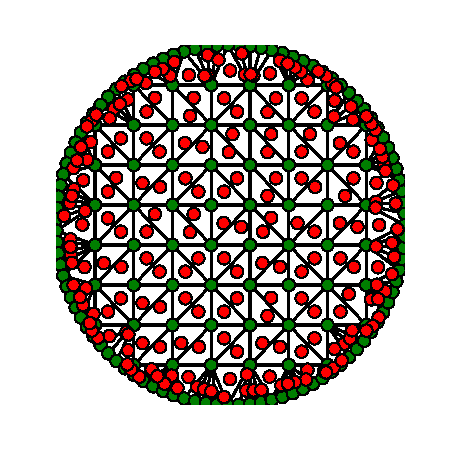
\includegraphics{figs/backmatter/meshCircle-100.pdf}
	\caption[Typical Delaunay triangulation mesh]
			{A typical mesh produced by the Delaunay triangulation.
			Here, 100 points were distrubuted along the boundary,  
			with another 100 inside the perimeter of the cavity. The green
			dots represent the nodes of the mesh. The red dots are the centroids
			of each triangle.}
	\label{fig:app.numMethods.meshDelaunayCircle}
\end{figure}

Figures \ref{fig:app.numMethods.fields} shows the field intensity
inside the cavity when $\phi(\bo{r})=J_0(kn_0r)$, i.e. the only
eigenfunction with vanishing angular momentum. We see that the field
maintains its main features when a finer mesh is used, indicative
of the convergence of the method. 

\begin{figure}
	\centering
	\begin{subfigure}{0.47\textwidth}
		\centering
		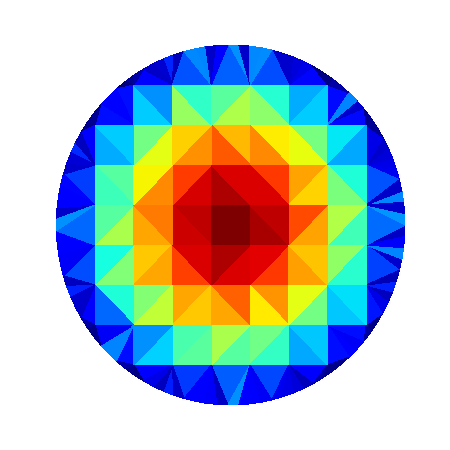
\includegraphics[width=\textwidth]{figs/backmatter/intensityTest-100.pdf}
		\caption[Intensity of the field inside the cavity]
				{Intensity of the field inside the cavity when
				$J_0(n_0kr)$ is the incoming field. This mesh contains
				100 points on the boundary and 100 more inside the perimeter.}
		\label{fig:app.numMethods.field.100}
	\end{subfigure}
	\hfill
	\begin{subfigure}{0.47\textwidth}
		\centering
		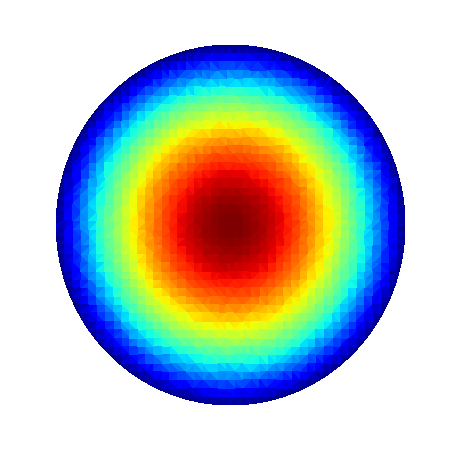
\includegraphics[width=\textwidth]{figs/backmatter/intensityTest-2000.pdf}
		\caption[Intensity of the field inside the cavity, finer mesh]
				{Intensity of the field inside the cavity when
				$J_0(kn_0r)$ is the incoming field. This mesh contains
				2000 points on the boundary and 2000 more inside the perimeter.}
		\label{fig:app.numMethods.field.2000}
	\end{subfigure}
	\caption[Intensity of the field inside the cavity for two different meshes]
			{Intensity of the field inside the cavity for two different meshes.
			We use $\phi(\bo{r})=J_0(kn_0r)$ as the incoming field.}
	\label{fig:app.numMethods.fields}
\end{figure}

The convergence is confirmed to be linear in the average area in 
the triangles in Figure \ref{fig:app.numMethods.convergenceIntegralMethod}.
The fact that it is slightly slower than linear can probably be 
attributed to the fact that we have neglected the diagonal 
parts of the kernel. 

\begin{figure}
	\centering
	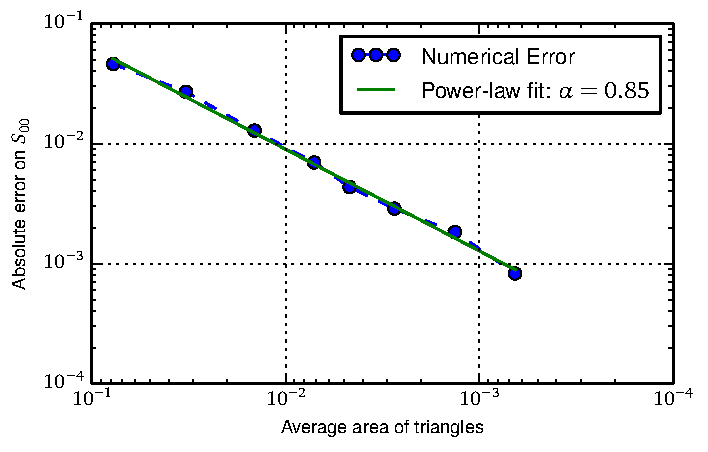
\includegraphics{figs/backmatter/convergenceAnalysis.pdf}
	\caption[Convergence analysis of the integral method]
			{Convergence analysis of the integral method. 
			We compute the difference between the analytical
			and numerical values of $S_{00}(k)$ for the homogeneous,
			circular cavity. The parameters are $k=1$, $R_0=1$, $n_c=1.5$
			and $n_0=1$.}
	\label{fig:app.numMethods.convergenceIntegralMethod}
\end{figure}

\section{Lippmann-Schwinger Computation of the Scattering Matrix: Vector Case}
We repeat the procedure of the previous section, but for the complete 3D vector
field. Similar methods are presented in \cite{deL2013,FAL2013}. As always, 
our starting point is the couple
	\begin{align}
		\nabla\times\bo{E}	& =ik\mu\bo{H}	& \nabla\times\bo{H}	&=-ik\epsilon\bo{E}.
	\end{align}
Taking the curl of the first equation and going through the motions, 
we can obtain the equation
	\begin{align}
		\label{eq:app.numMethods.LS.inhomogeneousPDE}
		\nabla^2\bo{E}+k^2\epsilon_\text{B}\mu_\text{B}\bo{E}	&=	-k^2\mu_\text{B}\Delta\epsilon\bo{E}
																	+\nabla\left\{\frac{1}{\epsilon_c}\bo{E}\cdot\nabla\epsilon_c\right\}	
																	+\mu_\text{B}\nabla\times\left(\Delta\mu^{-1}\nabla\times\bo{E}\right)
	\end{align}
where $\mu_\text{B}$ and $\epsilon_\text{B}$ are the permeability and permittivity
of the environment and where the supports of the functions
	\begin{align}
		\Delta\epsilon &= \epsilon_c-\epsilon_\text{B}	&	\Delta\mu^{-1}	&=\mu_c^{-1}-\mu_\text{B}^{-1}
	\end{align}
are supposed to coincide with the cavity region $\mathcal{C}$, 
with, now, $\mathcal{C}\subset\mathbb{R}^3$. $\epsilon_c$ 
and $\mu_c$ are the physical parameters of the cavity 
region and allowed to be non-linear, position- and frequency-dependent.
Once again, we have to solve an inhomogeneous partial differential equation.
We will use the tensorial Green's function\footnote{In the literature, it is called a dyadic 
Green's function. This nomenclature is archaic and should not be used in 
modern texts.}, given by \cite{NOV2012}
	\begin{equation}
		\mat{G}(\bo{r}',\bo{r}') = -\mat{I}\frac{e^{ikn_\text{B}|\bo{r}-\bo{r}'|}}{4\pi|\bo{r}-\bo{r}'|}.
	\end{equation}
where $n_B=\sqrt{\epsilon_B\mu_B}$. We can thus write a formal solution 
to the scattering problem as
	\begin{equation}
		\bo{E}(\bo{r}) = \bo{E}^i(\bo{r})
						+\mathop{\iiint}_\mathcal{C}\mat{G}(\bo{r},\bo{r}')\left[V(\bo{r}')\bo{E}(\bo{r}')\right]d^3\bo{r}'
	\end{equation}
where we have written the r.h.s. of \eqref{eq:app.numMethods.LS.inhomogeneousPDE}
as the operator
	\begin{equation}
		V(\bo{r})\{\} = -k^2\mu_B\Delta\epsilon\left\{\right\}
					+\nabla\left\{\frac{1}{\epsilon_c}\left\{\right\}\cdot\nabla\epsilon_c\right\}
					+\mu_B\nabla\times\left(\Delta\mu^{-1}\nabla\times\left\{\right\}\right).
	\end{equation}
Once again, this Lippmann-Schwinger equation can be used to compute the scattering tensor
of the problem. If we use the eigenfunction as the incoming field, we have
	\begin{equation}
		\bo{E}(\bo{r}) = j_L(n_Bkr)\bo{Y}^L_{JM}(\theta,\varphi)
						+\mathop{\iiint}_\mathcal{C}\mat{G}(\bo{r},\bo{r}')\left[V(\bo{r}')\bo{E}(\bo{r}')\right]d^3\bo{r}'
	\end{equation}
where the vector spherical harmonics are given by a combination of the
scalar spherical harmonics
	\begin{equation}
		\bo{Y}^\ell_{jm} = \sum_{m'}\sum_{\sigma}C^{jm}_{lm',1\sigma}Y_\ell^{m'}(\theta,\varphi)\bou{e}_\sigma
	\end{equation}
where $C^{j_3m_3}_{j_1m_1,j_2m_2}$ are the Clebsch-Gordan coefficients and where
the $\bou{e}_\sigma$ are the unit vectors of the covariant spherical coordinate system \cite{VAR1988}.
We will use the expansion
	\begin{align}
		\mat{G}(\bo{r},\bo{r}')	&= -ik\sum_{j,\ell,m} j_\ell(n_Bkr_<)h^{(+)}_\ell(n_Bkr_>)
													\bo{Y}^{\ell}_{jm}(\theta,\varphi)\otimes\bo{Y}^{\ell*}_{jm}(\theta',\varphi').
	\end{align}
Using the same technique as before, i.e. substituting the expansion in the integral equation
for the field outside the \gls{lss} and invoking the definition of the scattering matrix, 
we obtain
	\begin{equation}
		S_{j\ell m,JLM} = \delta_{j\ell m,JLM}
			-2ik\mathop{\iiint}_\mathcal{C}j_\ell(kn_Br')\bo{Y}^{j*}_{\ell m}V(\bo{r}')\bo{E}(\bo{r}')d^3\bo{r}'.
	\end{equation}
To compute the scattering tensor, however, we must necessarily solve an integro-differential equation.
We will not delve into the subject, as it is beyond the scope of this essay. However, 
it could be solved via a Galerkin method. 

The curl-curl equation yields a simple integral method when the material
is non-magnetic, but it seems impossible to recover our simple expression
for the scattering tensor.